\resizebox {.24\columnwidth} {!} {
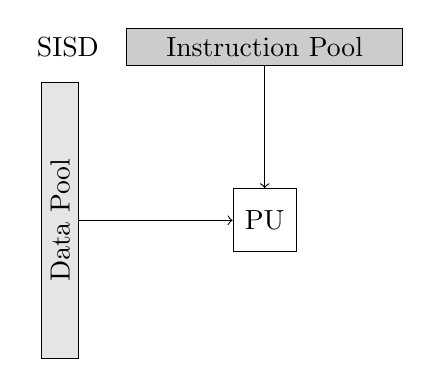
\begin{tikzpicture}
\draw (0.1,5.2) node {SISD}; 
\node (rect) at (2.6,5.2) [draw,minimum width=3.5cm,fill=black!20] (ip) {Instruction Pool};
\node (rect) at (0,3) [rotate=90,draw,minimum width=3.5cm,fill=black!10] (dp) {Data Pool};
\node (rect) at (2.6,3) [draw,minimum width=.8cm,minimum height=.8cm] (pu1) {PU};
\draw [->] (ip) -- (pu1);
\draw [->] (dp) -- (pu1);
\end{tikzpicture}
}
\resizebox {.24\columnwidth} {!} {
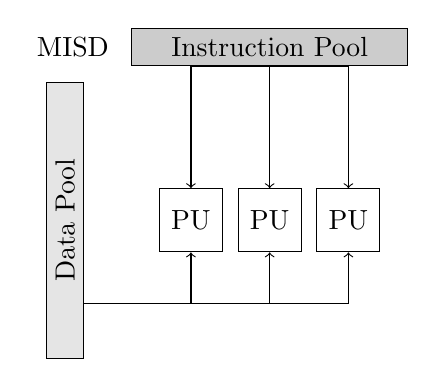
\begin{tikzpicture}
\draw (0.1,5.2) node {MISD}; 
\node (rect) at (2.6,5.2) [draw,minimum width=3.5cm,fill=black!20] (ip) {Instruction Pool};
\node (rect) at (0,3) [rotate=90,draw,minimum width=3.5cm,fill=black!10] (dp) {Data Pool};
\node (rect) at (1.6,3) [draw,minimum width=.8cm,minimum height=.8cm] (pu1) {PU};
\node (rect) at (3.6,3) [draw,minimum width=.8cm,minimum height=.8cm] (pu2) {PU};
\node (rect) at (2.6,3) [draw,minimum width=.8cm,minimum height=.8cm] (pu3) {PU};

\draw[<-] (pu1.north) |-  (ip.south); 
\draw[<-] (pu2.north) |-  (ip.south);
\draw[<-] (pu3.north) |-  (ip.south);

\draw[<-]  (pu1.south) |- ([yshift=-30pt]dp.south);
\draw[<-]  (pu2.south) |- ([yshift=-30pt]dp.south);
\draw[<-]  (pu3.south) |- ([yshift=-30pt]dp.south);

\end{tikzpicture}
}
\resizebox {.24\columnwidth} {!} {
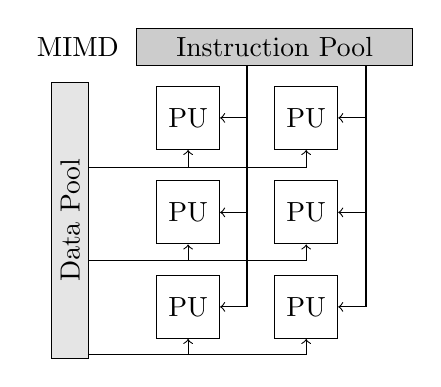
\begin{tikzpicture}
\draw (0.1,5.2) node {MIMD}; 
\node (rect) at (2.6,5.2) [draw,minimum width=3.5cm,fill=black!20] (ip) {Instruction Pool};
\node (rect) at (0,3) [rotate=90,draw,minimum width=3.5cm,fill=black!10] (dp) {Data Pool};
\node (rect) at (1.5,4.3) [draw,minimum width=.8cm,minimum height=.8cm] (pu1) {PU};
\node (rect) at (1.5,3.1) [draw,minimum width=.8cm,minimum height=.8cm] (pu2) {PU};
\node (rect) at (1.5,1.9) [draw,minimum width=.8cm,minimum height=.8cm] (pu3) {PU};
\node (rect) at (3,4.3) [draw,minimum width=.8cm,minimum height=.8cm] (pu4) {PU};
\node (rect) at (3,3.1) [draw,minimum width=.8cm,minimum height=.8cm] (pu5) {PU};
\node (rect) at (3,1.9) [draw,minimum width=.8cm,minimum height=.8cm] (pu6) {PU};

\draw[<-]  (pu1.south) |- ([yshift=19pt]dp.south);
\draw[<-]  (pu4.south) |- ([yshift=19pt]dp.south);

\draw[<-]  (pu2.south) |- ([yshift=-14.5pt]dp.south);
\draw[<-]  (pu5.south) |- ([yshift=-14.5pt]dp.south);

\draw[<-]  (pu3.south) |- ([yshift=-48.5pt]dp.south);
\draw[<-]  (pu6.south) |- ([yshift=-48.5pt]dp.south);

\draw[->] ([xshift=-10pt]ip.south) |- (pu1.east);
\draw[->] ([xshift=-10pt]ip.south) |- (pu2.east);
\draw[->] ([xshift=-10pt]ip.south) |- (pu3.east);

\draw[->] ([xshift=33pt]ip.south) |- (pu4.east);
\draw[->] ([xshift=33pt]ip.south) |- (pu5.east);
\draw[->] ([xshift=33pt]ip.south) |- (pu6.east);

%\draw[<-]  (pu2.south) |- ([yshift=-30pt]dp.south);
%\draw[<-]  (pu3.south) |- ([yshift=-30pt]dp.south);

%\draw [->] (ip) -- (pu1);
%\draw [->] (dp) -- (pu1);
\end{tikzpicture}
}
\resizebox {.24\columnwidth} {!} {
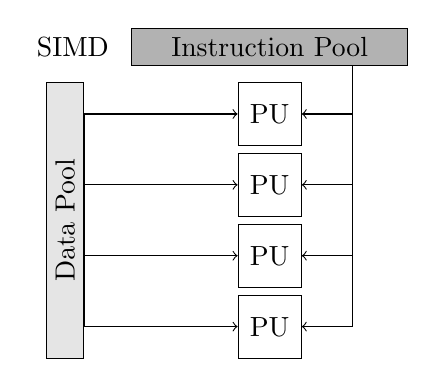
\begin{tikzpicture}
\draw (0.1,5.2) node {SIMD}; 
\node (rect) at (2.6,5.2) [draw,minimum width=3.5cm,fill=black!30] (ip) {Instruction Pool};
\node (rect) at (0,3) [rotate=90,draw,minimum width=3.5cm,fill=black!10] (dp) {Data Pool};
\node (rect) at (2.6,4.35) [draw,minimum width=.8cm,minimum height=.8cm] (pu1) {PU};
\node (rect) at (2.6,3.45) [draw,minimum width=.8cm,minimum height=.8cm] (pu2) {PU};
\node (rect) at (2.6,2.55) [draw,minimum width=.8cm,minimum height=.8cm] (pu3) {PU};
\node (rect) at (2.6,1.65) [draw,minimum width=.8cm,minimum height=.8cm] (pu4) {PU};
%\draw [->] ([yshift=2.35cm]dp) -- (pu1);
\draw[->] (dp.south) |- (pu1.west);
\draw[->] (dp.south) |- (pu2.west);
\draw[->] (dp.south) |- (pu3.west);
\draw[->] (dp.south) |- (pu4.west);

\draw[->] ([xshift=30pt]ip.south) |- (pu4.east);
\draw[->] ([xshift=30pt]ip.south) |- (pu3.east);
\draw[->] ([xshift=30pt]ip.south) |- (pu2.east);
\draw[->] ([xshift=30pt]ip.south) |- (pu1.east);
%\draw[arrow] (Small2B.north)--(Small2B|-Big2.south);s
%\draw [->] (dp) -- (pu1);
\end{tikzpicture}
}